\section{Related Work}
\label{sec:related_work}

\subsection{Data-driven Human Motion Synthesis}
Traditional human motion synthesis frameworks often rely on concatenative approaches such as \emph{motion graph} \cite{Kovar2002_MotionGraphs}. Recently, learning-based methods with neural networks have been widely applied to this area to generate high-quality and interactive motions, using models ranging from feed-forward network \cite{holden2017phase,Starke2022_DeepPhase} to dedicated generative models~\cite{henter2020moglow, Ling2020_MotionVAE}. Dealing with the one-to-many issue where a variety of motions can correspond to the same input or control signal is often a challenge for these learning-based approaches. Previous systems often employ additional conditions, such as contacts \cite{starke2020local} or phase indices \cite{holden2017phase,Starke2022_DeepPhase}, to deal with this problem. Closer to the gesture domain is the speech-driven head motion synthesis, where conditional GANs \cite{sadoughi2018novel}, and conditional VAEs \cite{greenwood2017predicting} have been used.

\subsubsection{Music-driven Dance Synthesis}
Among the general motion synthesis tasks, music-driven dance generation addresses a similar problem to the co-speech gesture synthesis, where the complex temporal relation between two different modalities needs to be modeled accurately. Both motion graph-based methods \cite{kim2006making,chen2021choreomaster} and learning-based approaches \cite{Li_2021_aist,valle2021transflower,li2022bailando} have been adopted and successfully achieved impressive generation results. To deal with the synchronization between the dance and music, \citet{chen2021choreomaster} develop a manually labeled rhythm signature to represent beat patterns and ensures the rhythm signatures of the generated dance match the music. \citet{aristidou2021rhythm} segment the dance into blocks at music onsets, convert each block into a motion motif \cite{aristidou2018deep} that defines a specific cluster of motions, and use the motion motif to guide the synthesis of dance at the block level. \citet{li2022bailando} employ a reinforcement learning scheme to improve the rhythmic performance of the generator using a reward function encouraging beat alignment. Our rhythm-based segmentation and canonicalization framework is partially inspired by \cite{aristidou2021rhythm}. Similar to \cite{aristidou2021rhythm}, we also segment the gestures into clips at audio beats but learn a high-level representation for each clip via the vector quantization scheme \cite{oord2017neural} instead of the K-means clustering. Moreover, our framework generates gestures in blocks of motion and denormalizes the generated motion blocks to match the rhythm of the speech. In contrast, \citet{aristidou2021rhythm} synthesize dance sequences in frames conditioned on the corresponding motion motifs.

\subsection{Co-speech Gesture Synthesis}
The most primitive approach used to generate human non-verbal behaviors is to animate an artificial agent using the retargeted motion capture data. This kind of approach is widely used in commercial systems (e.g., films and games) because of its high-quality motion performance. However, it is not suitable for creating interactive content that cannot be prepared beforehand. Generating co-speech gestures according to an arbitrary input has been a long-standing research topic. Previous studies can be roughly categorized into two groups, i.e., rule-based and data-driven methods.

\subsubsection{Rule-based Method}
The idea of the rule-based approach is to collect a set of gesture units and design specific rules that map a speech to a sequence of gesture units \cite{Kipp2004_Gesture, huang2012robot, softbank2018naoqi, cassell2004beat}. \citet{wagner2014gesture} have an excellent review of these methods. The results of the rule-based methods are generally highly explainable and controllable. However, the gesture units and rules typically have to be created manually, which can be costly and inefficient for complex systems.

\subsubsection{Data-driven Method}
Early research in data-driven method learns the rules embedded in data and combines them with predefined animation units to generate new gestures. For example, \citet{kopp2006towards, levine2010gesture} use probabilistic models to build correspondence between speech and gestures. \citet{Neff2008Gesture} build a statistical model to learn the personal style of each speaker. The model is combined with the input text tagged with the theme, utterance focus, and rheme to generate gesture scripts, which are then mapped to a sequence of gestures selected from an animation lexicon. \citet{chiu2015predicting} train a neural classification model to select a proper gesture unit based on the speech input. More recent research has started to take advantage of deep learning and trains  end-to-end models using raw gesture data directly, which frees the manual efforts of designing the gesture lexicon and mapping rules. Gestures can be synthesized using deterministic models such as multilayer perceptron (MLP) \cite{kucherenko2020gesticulator}, recurrent neural networks \cite{hasegawa2018evaluation, yoon2019robots, yoon2020speech, bhattacharya2021speech2affectivegestures, liu2022learning}, convolutional networks \cite{habibie2021learning}, and transformers \cite{9417647}, or by learning generative models such as normalizing flow \cite{alexanderson2020style}, VAEs \cite{li2021audio2gestures, xu2022freeform}, and learnable noise codes \cite{qian2021speech}. Our method is also a data-driven framework. We learn the motion generator and the mapping between the speech and gestures from data using a combined network structure of the vector quantized variational autoencoder (VQ-VAE)~\cite{oord2017neural} and LSTM. To capture the rhythmic and semantic correspondences between the speech and gestures, we propose a multi-stage architecture that explicitly models the rhythm and semantics in different stages. An earlier system proposed by \citet{kucherenko2021speech2properties2gestures} shares a similar high-level architectural design to our framework. However, there are two key differences: (a) our method is essentially an unsupervised learning approach, which learns the gesture lexeme, style code, and the generator directly from the data without detailed annotations; and (b) our system employs an explicit beat-based segmentation scheme which is shown to be effective in ensuring temporal coherence between the speech and the gesture.

\subsection{Multi-Modal Data Processing}
Co-speech gesture generation is a cross-modal process involving audio, text, motion, and other information related to the speaker and the content of the speech. The representation and alignment of each modality are essential for high-quality results~\cite{8269806}. Mel-spectrogram and MFCC acoustic features are commonly used as audio features \cite{alexanderson2020style, qian2021speech, kucherenko2020gesticulator}, typically resampled into the same framerate of the motion. For the text features, pre-trained language models like BERT \cite{devlin2019bert,kucherenko2020gesticulator} and FastText~\cite{bojanowski2017enriching,yoon2020speech} have been used to encode text transcripts into frame-wise latent codes, where paddings, fillers, or empty words are inserted into a sentence to make the world sequence the same length as the motion \cite{kucherenko2020gesticulator, yoon2020speech}. Speaker's style and emotions can also be encoded by learnable latent codes \cite{bhattacharya2021speech2affectivegestures,yoon2020speech} and are resampled or padded to match the length of the speech. In this work, we employ a pre-trained speech model to extract audio features and fine-tune it using a contrastive learning strategy. We also utilize a BERT-based model to vectorize the text. These multi-modal data are then aligned explicitly using the standard approaches discussed above. Notably, a concurrent study \cite{liu2022learning} also extracts audio features using contrastive learning. Their framework considers the learning of the audio features as a part of the training of the gesture generator. Instead, our framework trains the audio encoder in a separate pre-training stage using only the audio data.

\begin{figure*}[t]
    \centering
    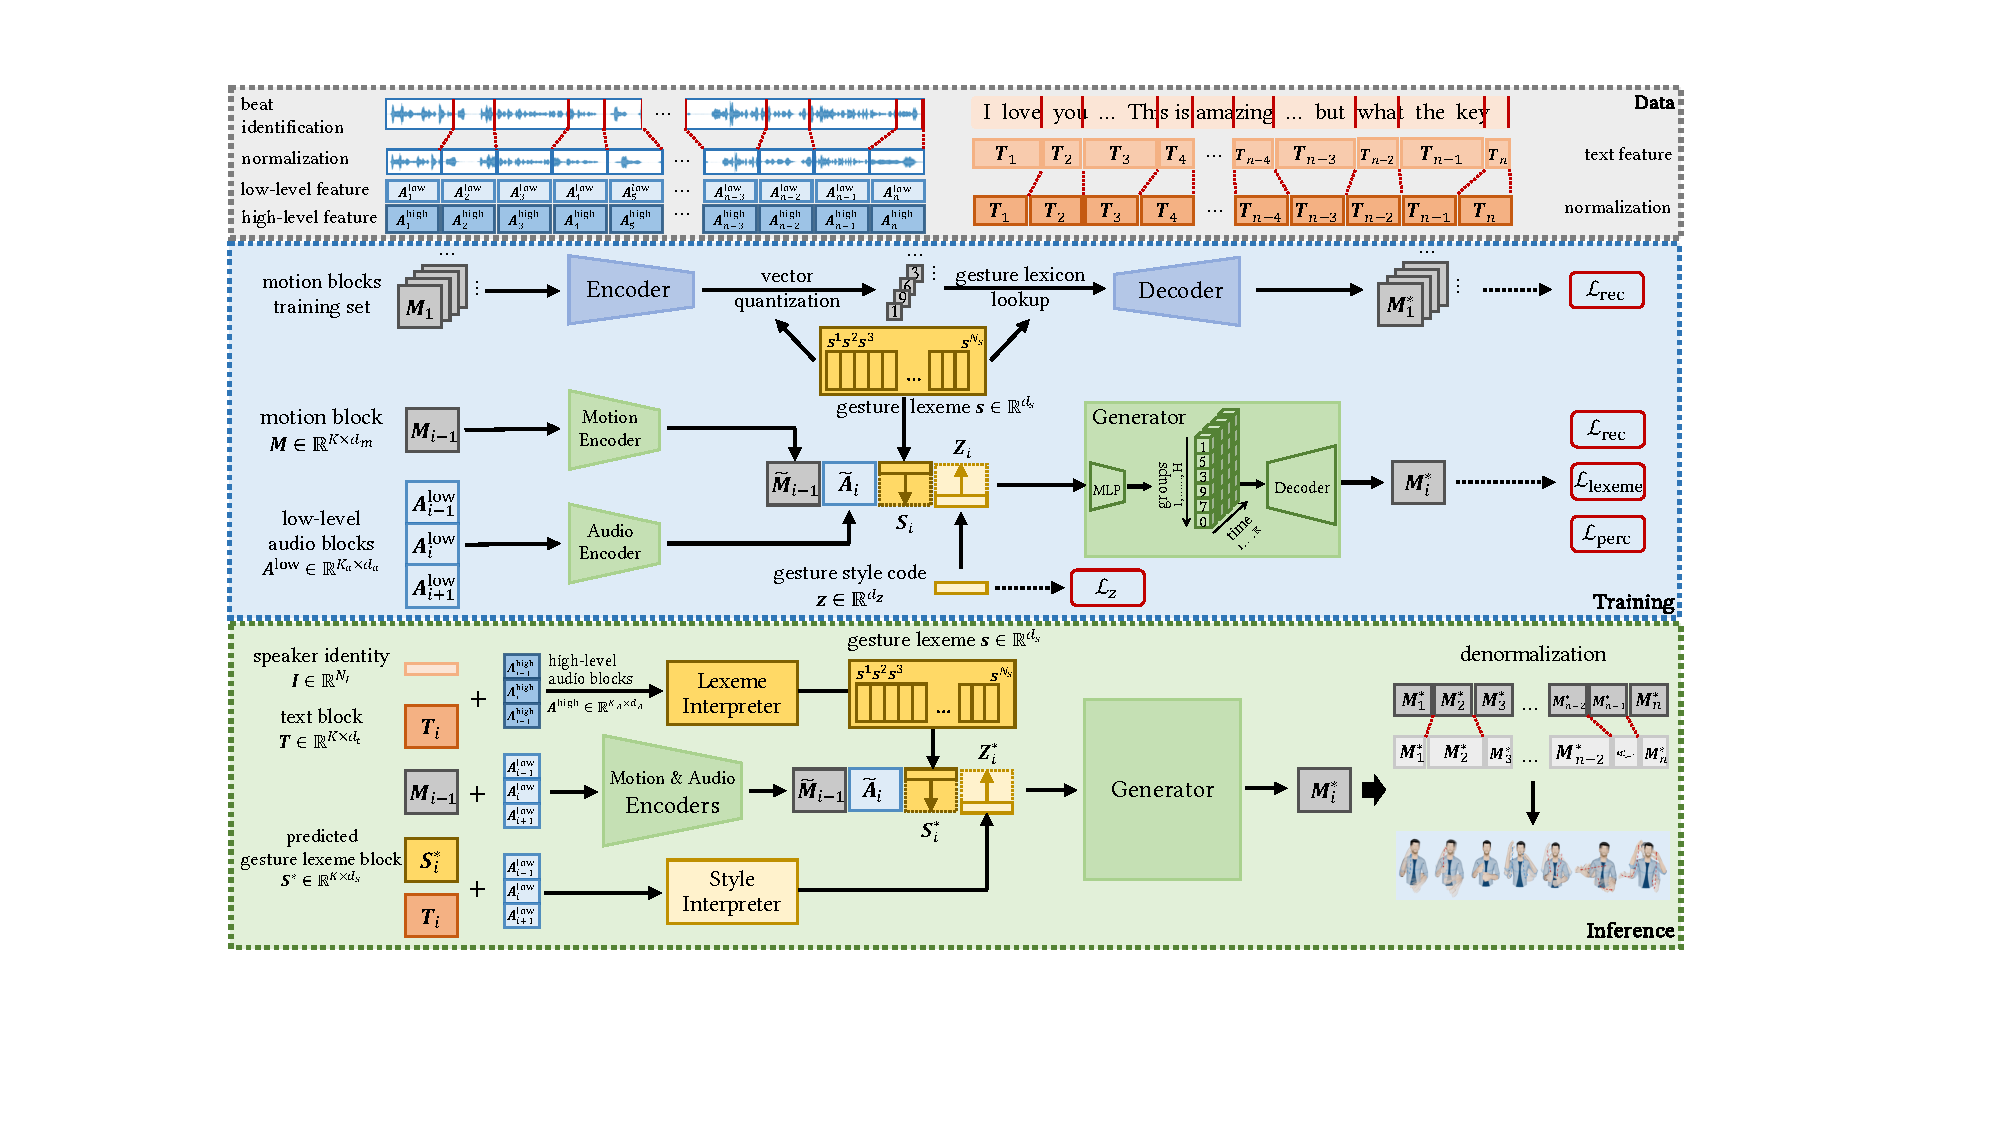
\includegraphics[width=\textwidth]{figures/overview.pdf}
    \caption{
    Our system is composed of three core components: 
    (a) the \emph{data} module preprocesses a speech, segments it into normalized blocks based on the beats, and extracts speech features from these blocks;
    (b) the \emph{training} module learns a gesture lexicon from the normalized motion blocks and trains the generator to synthesize gesture sequences, conditioned on the gesture lexemes, the style codes, as well as the features of previous motion blocks and adjacent speech blocks;
    and (c) the \emph{inference} module employs interpreters to transfer the speech features to gesture lexemes and style codes, which are then used by the learned generator to predict future gestures.
    }
    \Description{}
    \label{fig:system_overview}
\end{figure*}

\subsection{Evaluation of Motion Synthesis Models}
Evaluating the generated co-speech gestures is often difficult because the motion quality is a very subjective concept. Previous works have proposed several evaluation criteria. Wolfert et al.~\shortcite{wolfert2022evaluation} have made a comprehensive review of them. User studies are widely adopted to evaluate different aspects of motion quality, such as human-likeliness and speech-gesture matching \cite{alexanderson2020style, yoon2020speech, kucherenko2020gesticulator}, but can be expensive and hard to exclude uncontrolled factors. The absolute difference of joint positions or other motion features, such as velocity and acceleration between a reconstructed motion and the ground truth, is used by several works as an objective metric \cite{ginosar2019learning, joo2019towards, kucherenko2019analyzing}. However, this metric is not suitable for evaluating motions that are natural but not the same as the reference. Fr{\'e}chet Inception Distance (FID) \cite{heusel2017gans} is a widely used criterion in image generation tasks that measures the difference between the distributions of the dataset and generated samples in the latent space. It successfully reflects the perceptual quality of generated samples. Similarly, \citet{yoon2020speech} and \citet{qian2021speech} propose Fr{\'e}chet Gesture Distance (FGD) and Fr{\'e}chet Template Distance (FTD) metrics, respectively. These metrics measure the perceptual quality of generated gestures. In this paper, we compare our framework with several baseline methods using both user studies and objective metrics like FGD. We further propose a simple but effective rhythmic metric to measure the percentage of matched beats by dynamically adjusting the matching threshold, which provides a more informative picture of the rhythm performance.